\documentclass[10pt]{article}
% =========================================================
%                PAQUETES DE CONFIGURACIÓN
% =========================================================
\usepackage[T1]{fontenc}
\usepackage[utf8]{inputenc}
\usepackage[english,spanish]{babel}
\usepackage[
paperwidth=28cm,
paperheight=15.75cm,
top=0.20cm,
bottom=0.20cm,
left=0.40cm,
right=0.40cm
]{geometry}
\usepackage{xcolor}
\usepackage{setspace}
\usepackage{graphicx}
\usepackage{amsmath,amssymb}
\usepackage{hyperref}
\usepackage[many]{tcolorbox}
\usepackage{tikz}
\usetikzlibrary{shapes.geometric,calc}
\usepackage{ragged2e}
\usepackage{csquotes}
\usepackage{mathpazo}
\usepackage{microtype}
\usepackage{enumitem}

% =========================================================
%            ENTORNO PERSONALIZADO PARA EXTRACCIÓN A JS
% =========================================================
\newenvironment{extraer}[1]{}{}

% =========================================================
%                    CONFIGURACIÓN GENERAL
% =========================================================
\pagestyle{empty}
\setstretch{0.82}
\hypersetup{colorlinks=false}
\setlength{\parindent}{0pt}
\setlength{\parskip}{0pt}
\setlist{nosep,leftmargin=*}

% =========================================================
%                            COLORES
% =========================================================
\definecolor{deepblue}{RGB}{12,20,38}
\definecolor{gold}{RGB}{176,140,52}
\definecolor{golddark}{RGB}{120,90,22}
\definecolor{goldlight}{RGB}{225,205,145}
\definecolor{heartred}{RGB}{158,30,45}
\definecolor{burgundy}{RGB}{85,18,30}
\definecolor{textgray}{RGB}{35,33,30}
\definecolor{cream}{RGB}{253,250,244}
\definecolor{creamdark}{RGB}{244,237,222}
\definecolor{softgold}{RGB}{238,222,180}
\definecolor{framegold}{RGB}{162,128,42}

% =========================================================
%            SÍMBOLOS TIKZ (ULTRALIGEROS Y VECTORES)
% =========================================================
\newsavebox{\boxCruz}
\newsavebox{\boxCruzInvertida}
\newsavebox{\boxCorazonRojo}
\newsavebox{\boxCerebro}
\newsavebox{\boxCuantica}

\sbox{\boxCruz}{%
	\tikz[baseline=-0.35ex,scale=0.50]{
		\fill[golddark] (-0.09,0.42) rectangle (0.09,-0.48);
		\fill[golddark] (-0.28,0.18) rectangle (0.28,0.36);
		\fill[gold!88] (-0.07,0.40) rectangle (0.07,-0.46);
		\fill[gold!22] (-0.26,0.20) rectangle (0.26,0.34);
	}%
}
\sbox{\boxCruzInvertida}{%
	\tikz[baseline=-0.15ex,scale=0.50,rotate=180]{
		\fill[golddark] (-0.09,0.42) rectangle (0.09,-0.48);
		\fill[golddark] (-0.28,0.18) rectangle (0.28,0.36);
		\fill[gold!65] (-0.07,0.40) rectangle (0.07,-0.46);
		\fill[gold!65] (-0.26,0.20) rectangle (0.26,0.34);
	}%
}
\sbox{\boxCorazonRojo}{%
	\tikz[baseline=-0.25ex,scale=0.35]{
		\fill[heartred]
		(0,-0.55)
		.. controls (-0.55,-0.15) and (-0.55,0.45) .. (0,0.25)
		.. controls (0.55,0.45) and (0.55,-0.15) .. (0,-0.55);
		\fill[heartred!65!white,opacity=0.30]
		(-0.12,0.05) circle (0.11);
	}%
}
\sbox{\boxCerebro}{%
	\tikz[baseline=-0.2ex,scale=0.30]{
		\fill[burgundy]
		(0,0.55)
		.. controls (-0.55,0.55) and (-0.7,0.1) .. (-0.55,-0.25)
		.. controls (-0.4,-0.55) and (-0.15,-0.55) .. (0,-0.4)
		.. controls (0.15,-0.55) and (0.4,-0.55) .. (0.55,-0.25)
		.. controls (0.7,0.1) and (0.55,0.55) .. (0,0.55);
		\draw[cream,line width=0.65pt]
		(-0.35,0.15) .. controls (-0.1,0.35) and (0.1,0.0) .. (0.35,0.2);
		\draw[cream,line width=0.5pt]
		(-0.25,-0.15) .. controls (0.0,0.05) and (0.15,-0.25) .. (0.3,-0.05);
	}%
}
\sbox{\boxCuantica}{%
	\tikz[baseline=-0.3ex,scale=0.40]{
		\draw[golddark, line width=0.7pt, rotate=30] (0,0) ellipse (0.6cm and 0.25cm);
		\draw[golddark, line width=0.7pt, rotate=-30] (0,0) ellipse (0.6cm and 0.25cm);
		\draw[golddark, line width=0.7pt] (0,0) circle (0.35cm);
		\fill[gold!90] (0,0) circle (0.15cm);
		\fill[cream] (0,0) circle (0.06cm);
	}%
}

\newcommand{\cruz}{\usebox{\boxCruz}}
\newcommand{\cruzinvertida}{\usebox{\boxCruzInvertida}}
\newcommand{\corazonrojo}{\usebox{\boxCorazonRojo}}
\newcommand{\cuantica}{\usebox{\boxCuantica}}
\newcommand{\cerebro}{\usebox{\boxCerebro}}

% =========================================================
%                    MARCO DE LA PÁGINA
% =========================================================
\newcommand{\marcoPagina}{%
	\begin{tikzpicture}[remember picture,overlay]
		\fill[cream] (current page.south west) rectangle (current page.north east);
		\draw[framegold,line width=1.5pt]
		([xshift=0.25cm,yshift=-0.25cm]current page.north west)
		rectangle
		([xshift=-0.25cm,yshift=0.25cm]current page.south east);
		\draw[goldlight!80!gold,line width=0.5pt]
		([xshift=0.40cm,yshift=-0.40cm]current page.north west)
		rectangle
		([xshift=-0.40cm,yshift=0.40cm]current page.south east);
		\draw[gold!30,line width=0.25pt]
		([xshift=0.50cm,yshift=-0.50cm]current page.north west)
		rectangle
		([xshift=-0.50cm,yshift=0.50cm]current page.south east);
		\foreach \corner/\dx/\dy in {
			north west/0.25cm/-0.25cm,
			north east/-0.25cm/-0.25cm,
			south west/0.25cm/0.25cm,
			south east/-0.25cm/0.25cm
		}{
			\draw[gold!70!black,line width=0.8pt] ([xshift=\dx,yshift=\dy]current page.\corner) circle (4.0pt);
			\draw[goldlight,line width=0.35pt] ([xshift=\dx,yshift=\dy]current page.\corner) circle (5.5pt);
			\fill[golddark] ([xshift=\dx,yshift=\dy]current page.\corner) circle (1.5pt);
		}
	\end{tikzpicture}%
}

% =========================================================
%                    ESTILOS DE CAJAS
% =========================================================
\tcbset{
	sideStyle/.style={
		enhanced, colback=cream!98, colframe=gold!60!black,
		boxrule=0.7pt, arc=3pt, valign=center,
		left=2pt, right=2pt, top=1pt, bottom=1pt,
		borderline={0.2pt}{1.0pt}{gold!30}
	},
	titleBoxStyle/.style={
		enhanced, colback=gold!5!cream, colframe=gold!85!black,
		boxrule=0.9pt, arc=4pt, top=1.5pt, bottom=1.5pt, left=3pt, right=3pt,
		halign=center, borderline={0.3pt}{1.2pt}{gold!40}
	},
	contentStyle/.style={
		enhanced, colback=cream!99, colframe=gold!50!black,
		boxrule=0.7pt, arc=4pt, top=1.5pt, bottom=1.5pt, left=3pt, right=3pt,
		borderline={0.2pt}{1.0pt}{gold!22}
	},
	centralStyle/.style={
		enhanced, colback=cream!98, colframe=gold!60!black,
		boxrule=0.7pt, arc=4pt, top=1.5pt, bottom=1.5pt, left=3pt, right=3pt,
		borderline={0.25pt}{1.0pt}{gold!28}
	},
	introStyle/.style={
		enhanced, colback=cream!96, colframe=gold!55!black,
		boxrule=0.7pt, arc=4pt, top=2pt, bottom=2pt, left=3.5pt, right=3.5pt,
		borderline={0.25pt}{1.0pt}{gold!25}
	},
	finalQuoteStyle/.style={
		enhanced, colback=gold!7!cream, colframe=gold!80!black,
		boxrule=0.8pt, arc=3pt, top=1.5pt, bottom=1.5pt, left=3pt, right=3pt,
		halign=center, borderline={0.25pt}{1.0pt}{gold!40}
	}
}

% =========================================================
%                            DOCUMENTO
% =========================================================
\begin{document}
	\marcoPagina
	
	% 1. CABECERA SUPERIOR
	\noindent
	\begin{minipage}[c]{0.215\textwidth}
		\begin{tcolorbox}[sideStyle, width=\textwidth]
			\centering
			{\small\color{deepblue}\bfseries\begin{extraer}{condor_title}Cóndor del Sur\end{extraer}}\\[0.01cm]
			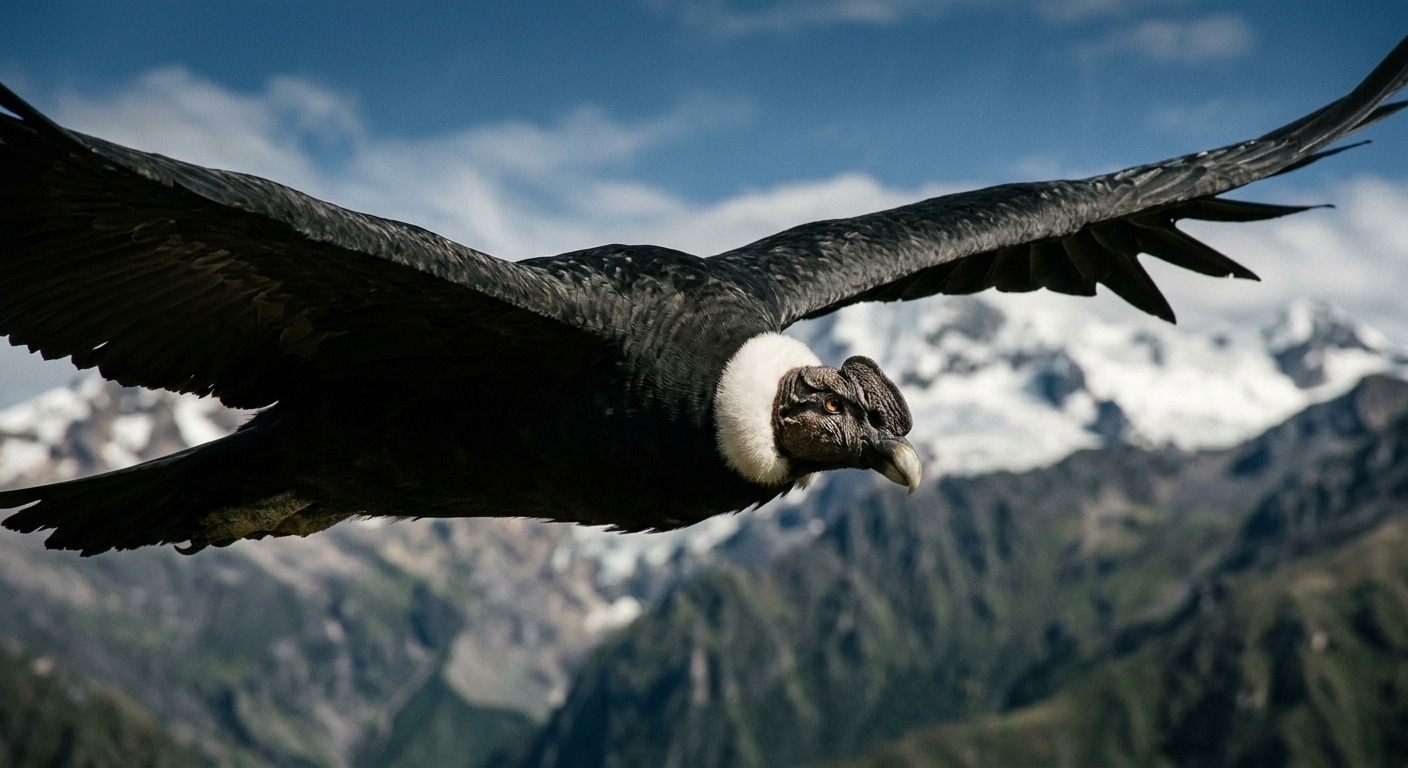
\includegraphics[width=\textwidth,height=1.35cm,keepaspectratio]{../images/TU_IMAGEN_CONDOR.jpg}\\[0.01cm]
			{\small\color{textgray}\itshape\begin{extraer}{condor_sub}Pneuma \corazonrojo: Intuición, espíritu y sentimiento divino \end{extraer}}
		\end{tcolorbox}
	\end{minipage}%
	\hfill
	\begin{minipage}[c]{0.55\textwidth}
		\begin{tcolorbox}[titleBoxStyle, width=\textwidth]
			\centering
			{\Large\color{deepblue}\bfseries\begin{extraer}{main_title}
					El Despertar \cruz 
			\end{extraer}}\\[0.01cm]
			\tikz[baseline=-0.5ex]{\draw[golddark, line width=0.7pt] (-2.2,0) -- (2.2,0); \fill[golddark] (0,0) circle (1.5pt);}\\[0.01cm]
			{\small\bfseries\color{golddark}\begin{extraer}{main_sub}Desde el pensamiento material al sentimiento divino \end{extraer}}
			
			\vspace{0.20cm}
			
			{\fontsize{7.4pt}{8.4pt}\selectfont 
				\begin{extraer}{header_desc}
					 El proyecto Divinidad y Conciencia Universal Cóndor y Águila busca trascender los dogmas medievales para comprender en profundidad nuestro verdadero lugar en el cosmos. Los seres humanos albergamos una Conciencia Dual y Cuántica. Atrapados en la prisión material de Yaldabaoth —el agujero negro en el que vivimos—, la humanidad tiene como vía de escape el despertar místico o el cruce de un puente de Einstein-Rosen: un agujero de pingüino de la conciencia que la transporta al Agujero Blanco: el Pléroma de Luz.
				\end{extraer}
			}
		\end{tcolorbox}
	\end{minipage}%
	\hfill
	\begin{minipage}[c]{0.215\textwidth}
		\begin{tcolorbox}[sideStyle, width=\textwidth]
			\centering
			{\small\color{deepblue}\bfseries\begin{extraer}{eagle_title}Águila del Norte\end{extraer}}\\[0.01cm]
			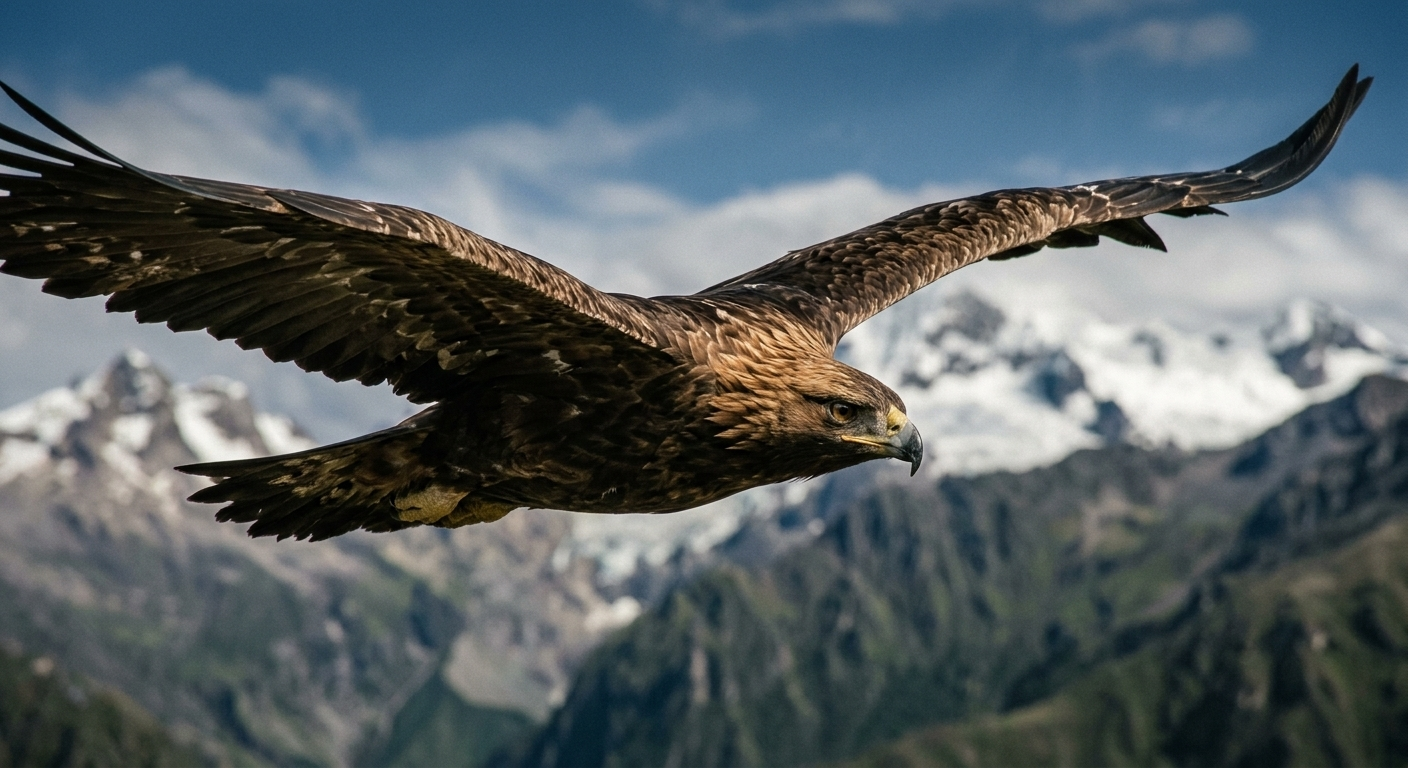
\includegraphics[width=\textwidth,height=1.35cm,keepaspectratio]{../images/TU_IMAGEN_AGUILA.jpg}\\[0.01cm]
			{\small\color{textgray}\itshape\begin{extraer}{eagle_sub}Psyche \cerebro: Ciencia, tecnología y pensamiento material\end{extraer}}
		\end{tcolorbox}
	\end{minipage}
	
	\vspace{0.03cm}
	
	% =========================================================
	% 2. BLOQUE 1: CONCIENCIA Y GRAVEDAD CUÁNTICA (ANCHO COMPLETO)
	% =========================================================
	\noindent
	\begin{tcolorbox}[introStyle, width=\textwidth]
		\begin{justify}{\fontsize{7.6pt}{8.8pt}\selectfont
				\setstretch{0.90}
				\centering{\bfseries\color{deepblue}\begin{extraer}{left_title}CONCIENCIA DUAL y  GRAVEDAD CUÁNTICA\end{extraer}}\\[0.10cm]
				\begin{extraer}{left_body}
					El universo es una autopista de dos carriles. Hoy transitas por el de la izquierda: el dominio de la materia, el pensamiento, la ciencia y la tecnología. Pero la Conciencia Primera nos convoca a despertar, recordándonos que en lo más profundo de nuestro ser arde una chispa sagrada. El carril de la derecha aguarda paciente: es el camino del espíritu, la intuición, el sentimiento divino. La solución a uno de los pilares fundamentales de la física moderna —la gravedad cuántica— halla su clave en escritos redactados hace casi dos milenios: los evangelios gnósticos. La conciencia se manifiesta a través de los estados $\vert \text{UNO} \rangle$ y $\vert \text{EGO} \rangle$, revelando que poseemos un auténtico libre albedrío de percepción, formalizado mediante el producto interno $\langle \text{UNO} \mid \text{EGO} \rangle$. El no-tiempo es una propiedad emergente de la pneuma, mientras que el espacio-tiempo es una propiedad emergente de la psyche. Dado que el ego humano posee masa, despojarnos de él equivale a trascender la densidad física: El EGO experimenta un Agujero Negro mientras que el UNO percibe un Agujero Blanco, trascendiendo la ilusión material para retornar a la luz del Padre Inefable
				\end{extraer}
		}\end{justify}
	\end{tcolorbox}
	
	\vspace{0.03cm}
	
	% =========================================================
	% 3. TRES COLUMNAS: UNIVERSO DE LUZ | IMAGEN | UNIVERSO MATERIAL
	% =========================================================
	\noindent
	\begin{minipage}[T]{0.25\textwidth}
		\begin{tcolorbox}[contentStyle, width=\textwidth]
			\centering
			{\normalsize\color{deepblue}\bfseries\begin{extraer}{universe_light_title}Universo de Luz\end{extraer}}\\[0.01cm]
			{\scriptsize\color{golddark}\bfseries\begin{extraer}{universe_light_sub}UNO \corazonrojo NoTiempo \cruz\end{extraer}}\\[0.01cm]
			\begin{justify}{\fontsize{6.7pt}{7.7pt}\selectfont\color{textgray}
					\begin{extraer}{universe_light_text}
						\textbf{El Padre y yo, uno somos}: Recordar quién eres —la revelación de que el Padre es el universo y de que la muerte no existe— nos libera de la ignorancia. En el hemisferio derecho reside el plano intemporal y divino, la dimensión de alta frecuencia $\vert 999\rangle$. Allí se encuentra la tierra de la unión y la libertad \textit{\textbf{(La Patria Grande)}}.
					\end{extraer}
			}\end{justify}
		\end{tcolorbox}
	\end{minipage}%
	\hfill
	\begin{minipage}[T]{0.50\textwidth}
		\begin{tcolorbox}[centralStyle, width=\textwidth]
			\centering
			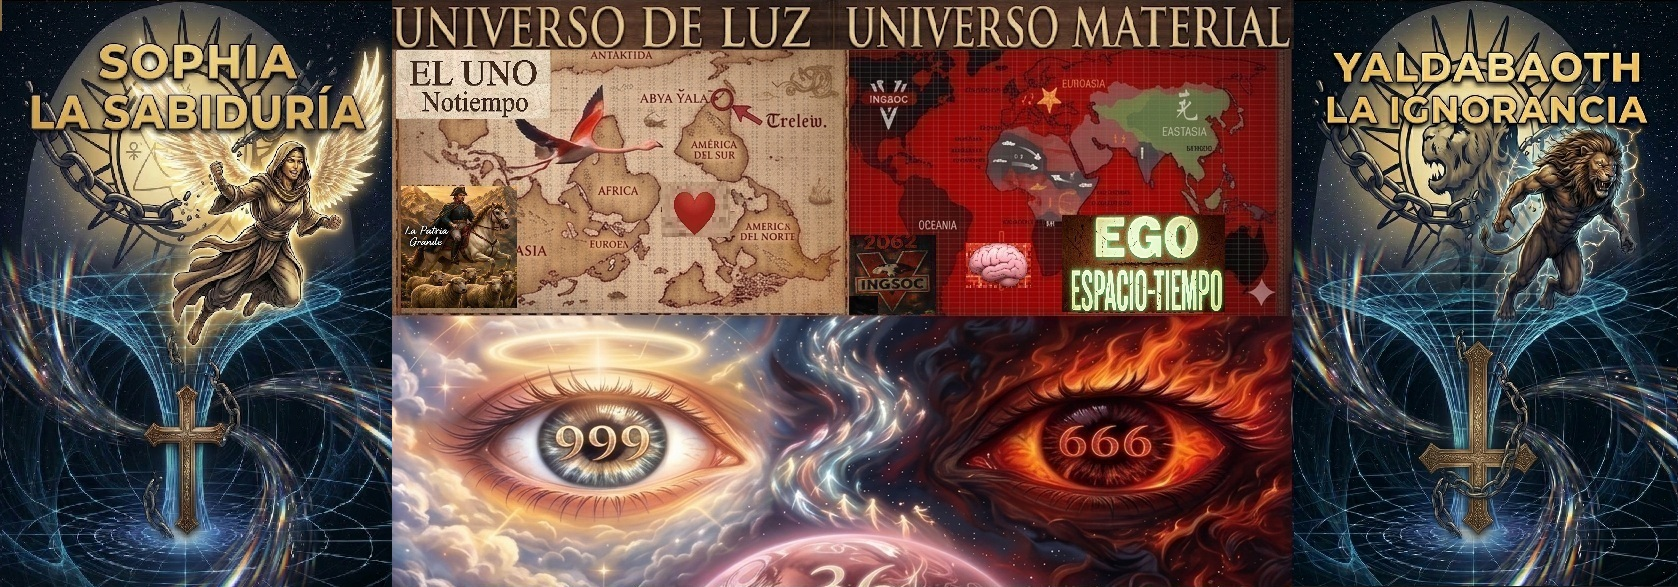
\includegraphics[width=\textwidth,height=3.50cm,keepaspectratio]{../images/sofiavsdemiurgo3.jpg}\\[0.01cm]
			{\scriptsize\color{golddark}\bfseries \begin{extraer}{center_text}
					Sofía, la sabiduría divina, yace atrapada en el caos del mundo material, gobernado por un demiurgo ignorante y cegado por su propio ego; donde el universo material se vincula al hemisferio del pensamiento y el Universo de Luz al del sentimiento reafirmando la máxima: \enquote{El Reino de Dios esta dentro de tí}.
			\end{extraer}}
		\end{tcolorbox}
	\end{minipage}%
	\hfill
	\begin{minipage}[T]{0.25\textwidth}
		\begin{tcolorbox}[contentStyle, width=\textwidth]
			\centering
			{\normalsize\color{deepblue}\bfseries\begin{extraer}{universe_mat_title}Universo Material\end{extraer}}\\[0.03cm]
			{\scriptsize\color{golddark}\bfseries\begin{extraer}{universe_mat_sub}EGO \cerebro espaciotiempo \cruzinvertida\end{extraer}}\\[0.01cm]
			\begin{justify}{\fontsize{6.7pt}{7.7pt}\selectfont\color{textgray}
					\begin{extraer}{universe_mat_text}
						El cuerpo humano está compuesto de carbono-12 ($6p^+$, $6e^-$, $6n^0$). En el hemisferio izquierdo radica el plano temporal y material, la dimensión de baja frecuencia $\vert 666\rangle$. La fuerza gravitacional del ego nos arrastran hacia un lugar donde: \enquote{la guerra es la paz, la libertad es la esclavitud y la ignorancia es la fuerza} (1984).
					\end{extraer}
			}\end{justify}
		\end{tcolorbox}
	\end{minipage}
	
	\vspace{0.03cm}
	
	\vspace{0.02cm}
	
	% =========================================================
	% 5. CITA FINAL Y PIE DE PÁGINA
	% =========================================================
	\begin{tcolorbox}[finalQuoteStyle, width=\textwidth]
		{\fontsize{9.5pt}{11.5pt}\selectfont\color{textgray}\itshape
			\enquote{\begin{extraer}{final_quote}Cuando el Águila del Norte y el Cóndor del Sur vuelen juntos en el mismo cielo, la Madre Tierra despertará y la humanidad entera sanará.\end{extraer}}}
	\end{tcolorbox}
	
	\vspace{0.1cm}
	
	\begin{center}
		\vspace{-0.2em}
		\hrule height 0.5pt
		\vspace{0.5em}
		\noindent{\small\textbf{\begin{extraer}{video_title}Documental \enquote{El Despertar \cruz: Desde el Pensamiento Material al Sentimiento Divino} \end{extraer}: } \url{https://www.condoryaguila.org}}
	\end{center}
	
\end{document}